\newpage
\section{Understanding Real-World Complexity Problems}
\label{sec:study}

In this section, we report an empirical study on real-world 
complexity problems. Our empirical study is conducted in two steps.

\begin{enumerate}

\item First, we build a taxonomy for studied complexity bugs. 
For bugs in each category, 
we study what code constructs conduct efficient computation,
how user-perceived slowdown is generated, and how to fix these bugs. 
Our studying results can help us 
make suitable design decisions for algorithmic profiling. 

\item Second, we investigate how these complexity problems are reported by end users
and how they are diagnosed by developers. 
This knowledge can help us understand what information is available from users' side
and help us understand the 
state of practice for combating complexity bugs.


\end{enumerate}

\subsection{Methodology}
\label{sec:meth}

\begin{table}[h!]
\centering
\small
\begin{tabular}{|@{\hspace{3pt}}l@{\hspace{3pt}}|@{\hspace{3pt}}c@{\hspace{3pt}}|}
\hline
Application Suite Description (language) & \# of Bugs\\
\hline                            
{\bf Apache Suite} 	                    & 4\\
%\cline{1-1}
{HTTPD:	Web Server (C)	}& \\
{TomCat:  Web Application Server (Java)}& \\
{Ant:	Build management utility (Java)}& \\
%\hline
%JMeter	& Load test utility (Java) & \\
\hline                            
{\bf Chromium Suite} Google Chrome browser (C/C++) & 3\\
\hline
%\multicolumn{2}{|l|}
{\bf GCC Suite}  GCC \& G++ Compiler (C/C++)     & 8\\
\hline
{\bf Mozilla Suite}  & 10\\
%\cline{1-1}
{Firefox: Web Browser (C++, JavaScript)}& 	\\
{Thunderbird: Email Client (C++, JavaScript)}& \\
\hline
{\bf MySQL Suite}     & 5	\\
%\cline{1-1}
{Server: Database Server (C/C++)}&  	\\
%\cline{1}
{Connector: DB Client Libraries (C/C++/Java/.Net)} &  	\\
\hline
{\bf Total}	   & \ComBugs \\
\hline
\end{tabular}
\caption{Applications and complexity bugs used in the study.}
\label{tab:app_bug}
\end{table}

We conduct our empirical study based on a public benchmark set of 
real-world performance bugs~\cite{PerfBug,SongOOPSLA2014}. 
In their first work~\cite{PerfBug}, 
the authors collected 110 real-world performance bugs from 5 representative 
software suites: Apache, Chrome, GCC, Mozilla, and MySQL. 
As shown in Figure~\ref{tab:app_bug}, 
these software suites cover various types of functionalities and are implemented 
in a variety of programming languages, including C/C++, Java, C\#, and JavaScript. 
All the five studied software suites are large and mature, 
with millions of lines of codes and long development histories. 
In their following work~\cite{SongOOPSLA2014}, 
the authors further identified 65 user-perceived performance bugs, 
whose bugs reports contain detailed information 
about how these bugs are perceived by end users and fixed by developers.  

Our study focuses on user-perceived complexity bugs, 
because these bugs have large performance impact.
After carefully reading bug reports and buggy code fragments 
associated with these bugs,
we clearly identify \ComBugs performance problems 
caused by {\textit{algorithmic complexity}}.
Developers usually fix these bugs by applying optimized algorithms to lower complexity
or to reduce workloads processed by buggy code fragments. 
We refer these performance problems as 
{\textit{complexity problems}} in the reminder of this paper.
The number of studied complexity problems are shown in Figure~\ref{tab:app_bug}.
Bugs not belonging to complexity problems are caused by various reasons.
For example, there are several Mozilla bugs related to GUI, 
like drawing transparent figures or refreshing web pages too frequently. 
There are also bugs caused by misusing synchronizations, 
such as using busy wait or conducting I/O in a critical section. 

{\bf{\textit{Caveats.}}}
In keeping with all previous empirical studies, 
our findings and conclusions need to be considered together with our methodology.
All studied complexity bugs come from software representative of a variety of uses and development processes. 
However, there are other types of software not covered in our study, 
such as distributed systems and software for high performance computation. 
All studied complexity problems are collected from bug databases.  
We believe that end users could report perceived complexity problems through other ways.
We also believe that there could be some complexity problems noticed 
and fixed by developers through manual inspection or in-house testing, 
before releasing the software to end users.  
However, the field has not found methods to study bugs not tracked by bug databases.
We believe that the studied bugs can serve as a representative sample
of complexity problems in the real world. 



\subsection{A Taxonomy for Complexity Problems}
\label{sec:tax}


%\begin{table*}
%\begin{adjustwidth}{-.5in}{-.5in}
%\small
%\centering
%{
%\begin{tabular}{|lcccccc|}
%\hline
%                                                               &   Apache  &   Chrome   &  GCC   &    Mozilla   &   MySQL  &  Total\\
%\hline
%Total \# of complexity bugs                                          &   4       &    3       &   8    &    10        &   5      &   30 \\
%\hline
%\multicolumn{7}{|c|}{\bf Taxonomy of complexity problems}\\
%\multicolumn{1}{|l}{{\bf $O(N)$}: linear complexity}                 &   1       &    0       &   0    &    4         &   3      &   8\\
%\multicolumn{1}{|l}{{\bf $O(N^k)$}: polynomial complexity (k>1)}     &   3       &    3       &   5    &    6         &   1      &  18\\
%\multicolumn{1}{|l}{{\bf $O(e^N)$}: exponential complexity}          &   0       &    0       &   3    &    0         &   1      &   4\\
%\hline
%\multicolumn{7}{|c|}{\bf How complexity problems are reported?}\\
%\multicolumn{1}{|l}{How to change input size {\bf is} specified}     &  4&2&5&9&5&25\\
%\multicolumn{1}{|l}{How to change input size {\bf not} specified}    &  0&1&3&1&0&5\\
%\hline
%\end{tabular}
%}
%\end{adjustwidth}
%\caption{Categorization for Section~\ref{sec:study}.
%(This table shows how complexity problems distribute among different complexity categories
% and whether or not how to change input size is specified during reporing.)}
%\label{tab:study}
%\end{table*}


\begin{table*}[tb!]
\begin{adjustwidth}{-.5in}{-.5in}
\small
\centering
{
\begin{tabular}{|lcccccc|}
\hline
                                                                                  &   Apache  &   Chrome   &  GCC   &    Mozilla   &   MySQL  &  Total\\
\hline
Total \# of complexity bugs                                                       &   4       &    3       &   8    &    10        &   5      &   30 \\
\hline
\multicolumn{7}{|c|}{\bf Taxonomy of complexity problems}\\
\multicolumn{1}{|l}{{\bf $O(N)$}: linear complexity}                              &   1       &    0       &   0    &    4         &   2      &   7\\
\multicolumn{1}{|l}{{\bf $O(N^k)$}: polynomial complexity ($k>1$)}                &   3       &    3       &   5    &    6         &   2      &  19\\
\multicolumn{1}{|l}{{\bf $O(e^N)$}: exponential complexity}                       &   0       &    0       &   3    &    0         &   1      &   4\\
\hline
\multicolumn{7}{|c|}{\bf How complexity problems are fixed?}\\
\multicolumn{1}{|l}{Optimize {\bf directly}: Buggy code is revised}              &  3        &    3       &   4    &    9         &   5      &  24 \\
\multicolumn{1}{|l}{Optimize {\bf indirectly}: Workloads are skipped}              &  1        &    0       &   4    &    1         &   0      &   6\\
\hline
\multicolumn{7}{|c|}{\bf How complexity problems are reported?}\\
\multicolumn{1}{|l}{Input size {\bf is} specified}                                &  4        &    2       &   4    &    9    &5   &24\\
\multicolumn{1}{|l}{Input size is {\bf not} specified}                            &  0        &    1       &   4    &    1    &0   &6\\
\hline
\end{tabular}
}
\end{adjustwidth}
\caption{Categorization for Section~\ref{sec:study}.
\footnotesize{(This table shows how complexity problems distribute among different complexity categories, how developers fix studied complexity problems,
 and whether or not how to change input size is specified during reporting.)}}
\label{tab:study}
% \vspace{-0.4in}
\end{table*}


After categorizing studied bugs according to their different complexity, 
we study complexity problems in each category.
Our study focuses on 
1) what are root causes\footnote{We refer root causes as code constructs 
conducting the inefficient computation, 
following previous works in this area~\cite{SongOOPSLA2014,ldoctor}.} 
for the complexity problems;
2) how the complexity problems generate user-perceived performance impact;
3) how developers fix these complexity problems. 

{\underline{\textit{$O(N)$: linear complexity.}}} 
As shown in Table~\ref{tab:study}, 
7 out of \ComBugs studied complexity problems are in linear complexity. 
All of these problems are caused by a buggy loop, 
whose average loop iteration number scales in terms of input size $N$.

Five of them are characterized by buggy loops that contain serialized I/O operations.
Users could perceive these bugs, 
even though the average loop iteration numbers of input sizes are not large.
Patching these 5 bugs involves aggregating I/O operations 
or completely eliminating unnecessary I/O operations. 
For example, Mozilla\#490742 is caused by bookmarking 
tabs by using individual database transactions. 
Even bookmarking 50 tabs can cause a timeout dialog 
window to pop up in a performance failure run. 
To fix this bug, Mozilla developers use one single aggregated transaction 
to bookmark all tabs.
As another example, Mozilla\#344059 is due to saving unchanged 
search engine preferences to SQLite, 
and it is fixed by saving search 
engine preferences only when some of them are changed.


For the other three bugs,
their buggy loops execute many iterations during performance failure runs.
They are fixed by adding shortcuts to completely skip the buggy loops. 
Taking MySQL\#33948 as an example,
MySQL developers followed a common practice to keep all table entries in the same linked list, 
including both used ones and free ones. 
The buggy loop iterates the linked list and looks for a free entry.
During performance failure runs, 
many table entries are used and the buggy loop must iterate excessively to find a free entry.
To fix this bug, MySQL developers simply separate used entries and free entries,
and keep them in two separated linked lists. 

To sum up, all $O(N)$ complexity problems are caused by buggy loops. 
To fix them, developers directly optimize these loops or completely skip these loops. 


%\begin{figure}
%\centering
%\lstset{basicstyle=\ttfamily\fontsize{7}{8}\selectfont,
%     morekeywords={+},keepspaces=true,numbers=left}
%  \mbox{\lstinputlisting[mathescape,boxpos=t]{figure/mysql27287.c}}
%\caption{A MySQL performance problem in polynomial complexity. 
%\footnotesize{(During performance failure runs, 
%   the total loop iterations scale polynomially in the size of \texttt{items}.)}}
%\vspace{-0.05in}
%\label{fig:mysql27287}
%\vspace{-0.05in}
%\end{figure}



{\underline{\textit{$O(N^k)$: polynomial complexity (k>1).}}}
As shown in Table~\ref{tab:study}, 
more than half of the studied complexity bugs are in polynomial complexity. 
Similar to complexity problems in linear complexity,
polynomial complexity for each problem is also caused by a buggy loop.
However, {\bf both} loop execution number and average loop iteration number
scale as input size $O(N)$.

\begin{figure}
\centering
\lstset{basicstyle=\ttfamily\fontsize{7}{8}\selectfont,
     morekeywords={+},keepspaces=true,numbers=left}
  \mbox{\lstinputlisting[mathescape,boxpos=t]{figure/Mozilla477564.js}}
\caption{A Mozilla complexity problem in $O(N^2)$ complexity.
\footnotesize{(This figure shows the buggy code fragment for Mozilla\#477564. 
Execution time scales polynomially in the number of nodes in a linked list.)}}
\vspace{-0.05in}
\label{fig:Mozilla477564}\vspace{-0.05in}
\end{figure}

\begin{figure*}
\centering
\subfloat[MySQL\#27287]{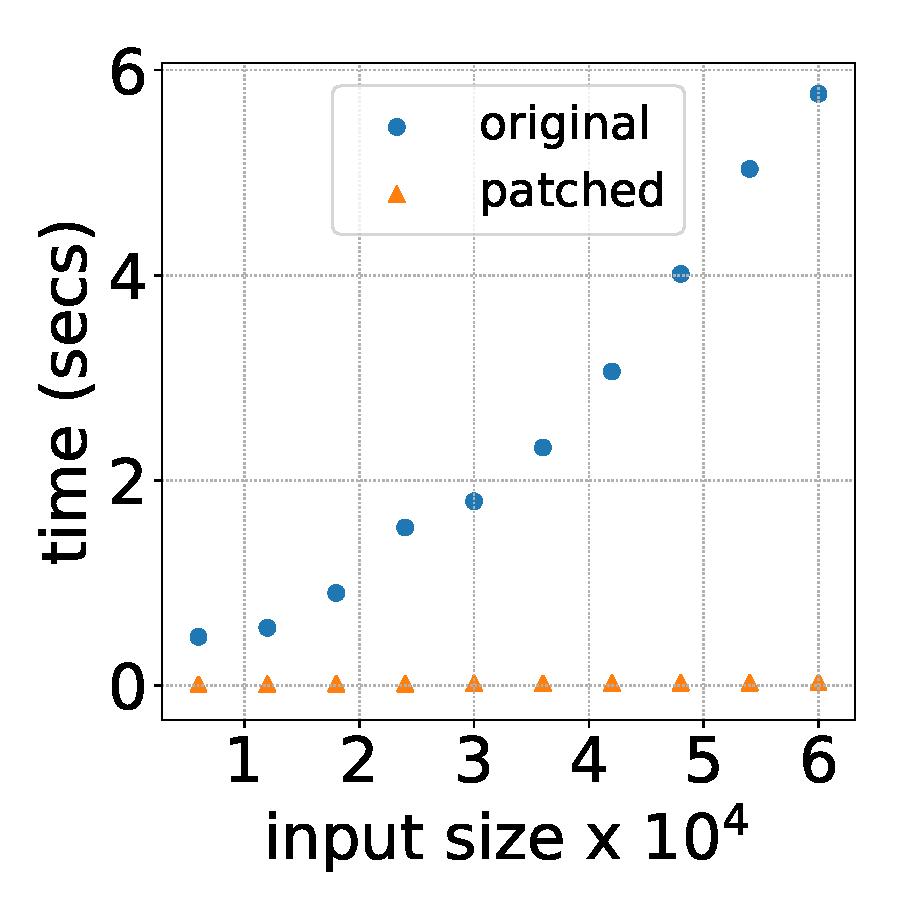
\includegraphics[width=0.22\linewidth]{figure/mysql27287-runtime-original-fixed-line}\label{fig:mysql27287-time}} 
\subfloat[Mozilla\#477564]{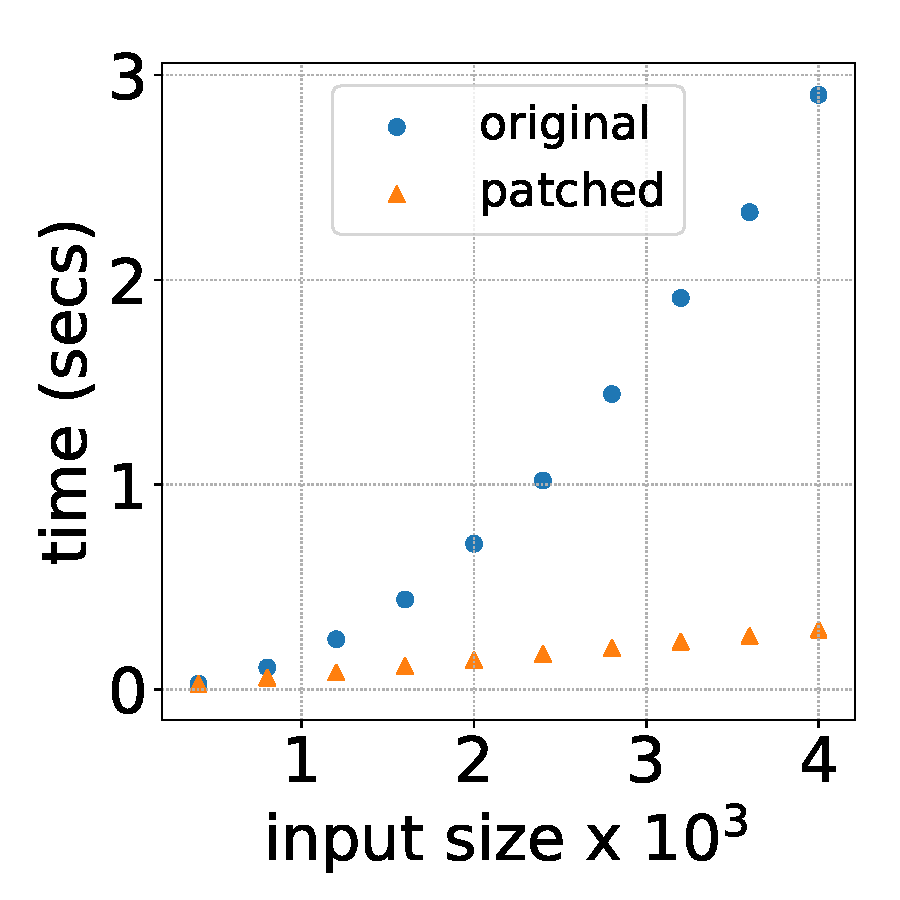
\includegraphics[width=0.22\linewidth]{figure/mozilla47564-runtime-original-fixed-line}\label{fig:mozilla477564-time}}
\subfloat[Apache\#34464]{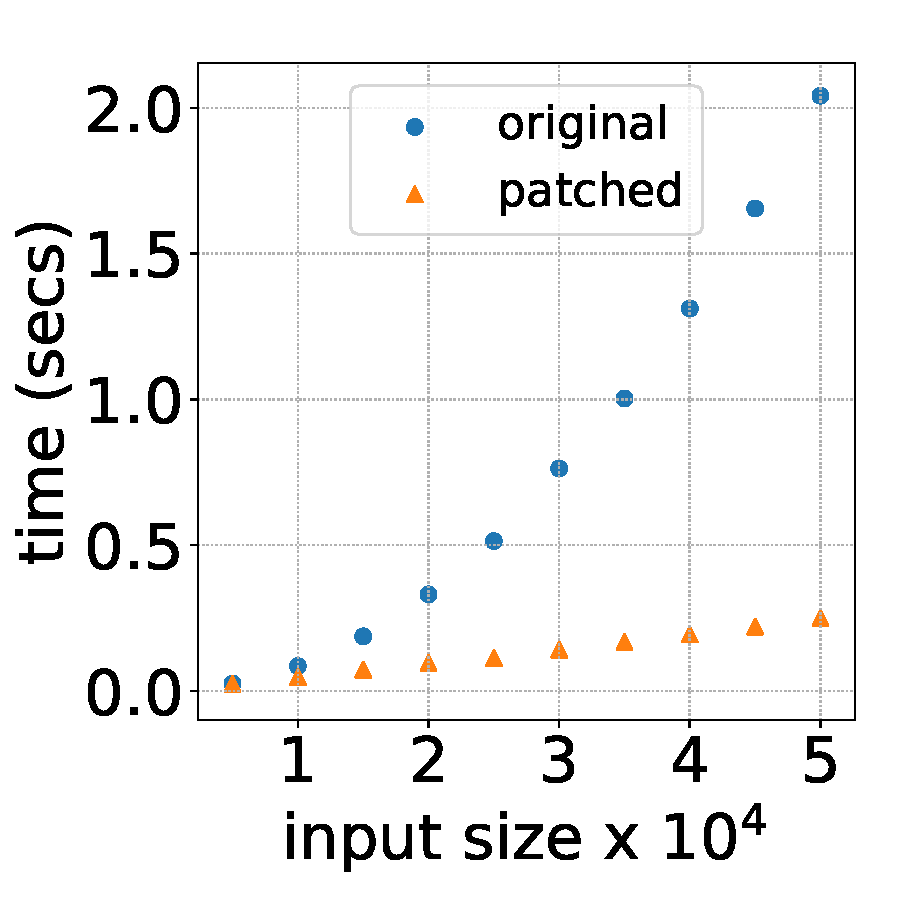
\includegraphics[width=0.22\linewidth]{figure/apache34464-runtime-original-fixed-line}\label{fig:apache34464-time}} 
\subfloat[GCC\#27733]{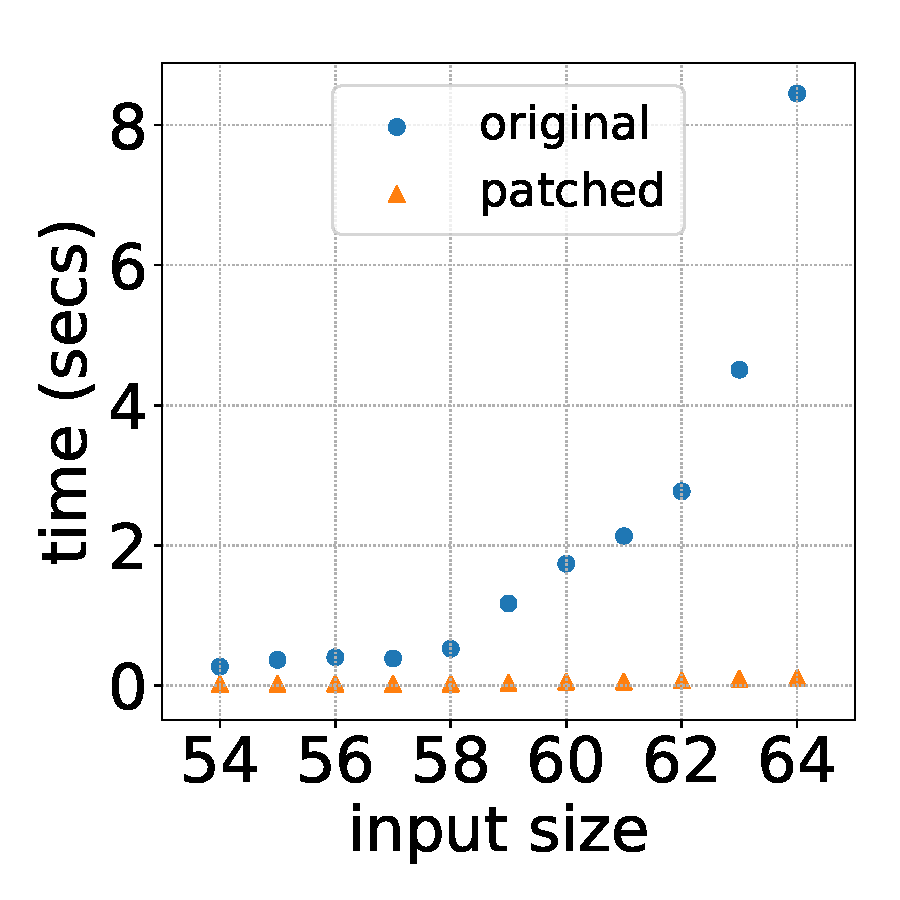
\includegraphics[width=0.22\linewidth]{figure/gcc27733-runtime-original-fixed-line}\label{fig:gcc27733-time}} \\ 
\vspace{-0.1in}
\caption{How execution time scales with input size for four complexity problems. 
\footnotesize{(These figures show how execution time change with the change of input size for MySQL\#27287, 
 Apache\#34464, Mozilla\#477564, and GCC\#27733. For each complexity problem, we use 10 distinct inputs.)}} 
\label{fig:time} 
\end{figure*} 

To fix the majority (14/19) of performance problems in this category,
developers directly modify the buggy loops, 
whose total loop iteration numbers scale polynomially.
Take MySQL\#27287 as an illustration.
As we discussed earlier, to fix this bug,
developers add an extra field to save parent \texttt{XML\_NODE}
and completely remove the buggy loop shown in Figure~\ref{fig:mysql27287}.
As another example, the buggy loop for Mozilla\#477564 is shown in Figure~\ref{fig:Mozilla477564}.
The loop counts how many previous nodes of input \texttt{aNode} 
having the same \texttt{localName} and \texttt{URI}.
An outer loop, not shown in the figure, 
will invoke \texttt{sss\_xph\_generate} for every node in a linked list, 
so that the complexity is $O(N^2)$ in terms of the number of nodes in the linked list.
To fix this complexity bug, developers add an extra field to each node to 
save the counting result. 
Given a node, 
its \texttt{count} value is calculated by adding one 
to the \texttt{count} value of 
its nearest previous node with the same \texttt{localName} and \texttt{URI}.  
How complexity changes after fix for MySQL\#27287 and Mozilla\#477564 are 
shown in Figure~\ref{fig:mysql27287-time} and Figure~\ref{fig:mozilla477564-time}, respectively. 

\begin{figure}
\centering
\lstset{basicstyle=\ttfamily\fontsize{7}{8}\selectfont,
     morekeywords={+},keepspaces=true,numbers=left}
  \mbox{\lstinputlisting[mathescape,boxpos=t]{figure/apache34464.c}}
\caption{An Apache performance problem in $O(N^2)$ complexity and its patch. 
\footnotesize{(This figure shows the buggy code fragment for Apache\#34464. 
 Execution time scales polynomially in the number of characters read from \texttt{getchar()}.)}}
\vspace{-0.05in}
\label{fig:apache34464}
\vspace{-0.05in}
\end{figure}





%To fix the majority (13/18) of performance problems in this category, 
%developers directly modify the loops whose total loop iterations scale polynomially.  
%The buggy loop for MySQL\#27287 is shown in Figure~\ref{fig:mysql27287}.
%The loop searches parent \texttt{XML\_NODE} for function parameter \texttt{nitems}, 
%which presents array index for another \texttt{XML\_NODE}.
%All \texttt{XML\_NODE}s are maintained in array \texttt{items}. 
%The way the loop to conduct the search is to iterate array \texttt{items} 
%backward from the input and look for the first \texttt{XML\_NODE} 
%whose level is one less than the input.
%During performance failure runs, 
%one \texttt{XML\_NODE} contains tens of thousands of children, 
%and \texttt{xml\_parent\_tag} is invoked for each of its children. 
%To fix this bug, MySQL developers add an extra field to each 
%\texttt{XML\_NODE} to save its parent, 
%and this field is initialized when a \texttt{XML\_NODE} is created. 
%After that, the buggy loop is completely removed. 


To fix other complexity problems (5/19) in this category,
developers reduce data processed by the loops scaling polynomially, 
instead of changing the loops directly.
In the buggy code fragment for Apache\#34464 shown in Figure~\ref{fig:apache34464},
the \texttt{while} loop on line 5 searches a string \texttt{source}
for a target sub-string \texttt{target}.
If the \texttt{while} loop's search is unsuccessful, 
a new character returned from \texttt{getchar()} on line 8 will be appended to string \texttt{source}, 
and the loop will search string \texttt{source} again from the beginning. 
There is an inner loop inside \texttt{indexOf()}, whose total iterations 
scale polynomially in terms of the number of characters from \texttt{getchar()}. 
After fixing this bug, the inner loop will only check the most recent \texttt{targetLen} characters.
The developers not change the inner loop, 
while reduce the workload it processes.   
How execution time scales before and after fix for 
Apache\#34464 is shown in Figure~\ref{fig:apache34464-time}.
Take GCC\#12322 as another example.
The loop scaling polynomially is part of the functionality that does basic block reordering,
and it will perform poorly for basic blocks with too many successors. 
The bug-triggering input contains a basic block with thousands of successors. 
To fix this, developers simply skip basic blocks with many successors.
By does this, some optimization opportunities may be lost, 
but the generated codes will still work correctly. 


{\underline{\textit{$O(e^N)$: exponential complexity.}}}
Four of the studied complexity problems are in exponential complexity. 
These complexity problems are fixed 
either by leveraging memoization to reuse previous results 
or by skipping computation with exponential complexity for large workloads. 



\begin{figure}
\centering
\lstset{basicstyle=\ttfamily\fontsize{7}{8}\selectfont,
     morekeywords={+},keepspaces=true,numbers=left}
  \mbox{\lstinputlisting[mathescape,boxpos=t]{figure/gcc27733.c}}
\caption{A GCC performance problem in exponential complexity. 
 \footnotesize{(During performance failure runs, how many times \texttt{mult\_alg} is invoked scales exponentially
  in the number of 1s in the binary form of input \texttt{t}.)}}
\vspace{-0.05in}
\label{fig:gcc27733}
\vspace{-0.05in}
\end{figure}


Three of the studied performance problems are caused by recursive function calls. 
Taking GCC\#27733 in Figure~\ref{fig:gcc27733} as an example, 
the recursive function \texttt{mult\_alg} computes the best algorithm to multiply \texttt{t}.
In each invocation, \texttt{mult\_alg} will try a set of bitwise 
operations to change input 
\texttt{t} into a smaller number, \texttt{t'}, 
and recursively call itself.
The number of times when \texttt{mult\_alg} is invoked scales exponentially 
in terms of the number of 1s in the binary form of input \texttt{t}.
To optimize this function, 
GCC developers use a hash table, \texttt{alg\_hash}, to record
which \texttt{t} has been processed before and its corresponding result.
However, there is a type declaration error inside the hash table entry,
and this error causes \texttt{t} larger than the maximum unsigned integer to never hit cache.
For large \texttt{t}, \texttt{mult\_alg} is still in exponential complexity. 
After fixing the type declaration error, 
memoization is enabled for large \texttt{t}. 

GCC\#32540 is in the exponential complexity category and is caused by an inefficient loop. 
The loop applies an iterative algorithm to implement a compiler optimization. 
The bug-triggering input contains very complex control and data dependence,  
so that the buggy loop scales exponentially in terms of the number 
of \texttt{if} branches in the input. 
To fix this bug, developers simply disable the optimization 
once they detect the complex control and data dependence.  


\subsection{Diagnosis process of complexity problems}
\label{sec:process}

We also studied how complexity problems are reported by users 
and get diagnosed by developers 
to better understand state-of-the-art combating process for complexity problems. 

{\underline{\textit{How are complexity problems reported?}}
As shown in Table~\ref{tab:study},
for most complexity bugs (24/30), 
users' reports specify how to change input sizes 
in order to observe the performance scaling problems. 
As discussed in previous works~\cite{SongOOPSLA2014}, 
all collected user-perceived performance-bug reports
contain bug-triggering inputs from end users. 
For most complexity bugs, 
users also describe how they change input sizes 
and how performance changes accordingly. 
For example, when reporting GCC\#32540, 
the user provides a C file and several measurement results to 
show that GCC compilation time scales exponentially 
with the number of \texttt{if} branches in the C file. 
As another example, when reporting Mozilla\#490742, 
the user mentions that the length of high, 
flat CPU usage is related to the number of search engine preferences. 


For the other five bugs, users provide one bug-triggering input 
or describe a set of bug-triggering inputs when they report the complexity problems. 
For example, when reporting GCC\#27733, 
the user provides one bad input, which can take GCC 49 minutes to compile. 
When reporting Mozilla\#231300, the user mentions 
that clearing the disk cache on a Macintosh system can trigger the bug, 
regardless of the content of the cached files. 


{\underline{\textit{How complexity problems are diagnosed?}}
We studied how long it takes developers to fix complexity problems. 
On average, it takes developers 162 days to diagnose a complexity problem. 
Following the same methodology as the previous work~\cite{SongOOPSLA2014},
we calculate diagnosis time as starting from when a problem 
was reported to a bug tracking system
and ending when a correct patch was submitted on the bug tracking system. 
On average, it takes developers 101 days to diagnose non-complexity bugs in the same performance-bug set. 
Diagnosing complexity problems takes longer time.
After separating bugs from different applications, 
we observe that developers consistently need more time to diagnose complexity problems.
%compared with non-complexity bugs.
Among the five applications, 
Chrome developers need 4.5 times longer to diagnose complexity problems,
which is the maximum increase.
MySQL developers spend most similar time to diagnose complexity problems,
while the time they spend is still 0.43 times longer. 

As discussed in the previous works~\cite{SongOOPSLA2014}, 
traditional profilers are the only type of diagnosis tools mentioned in bug reports 
when diagnosing the collected user-perceived performance problems. 
Tradisional profilers are mentioned in 7 out of 30 complexity-bug reports. 
A similar percentage of bug reports mention traditional profilers
when comparing complexity bugs with non-complexity bugs. 

\subsection{Implications}

{\underline{\textit{Implication 1}}
The patches for most studied complexity problems (24/30)
are designed to directly optimize loops or recursive functions that scale poorly.
Accurately attributing complexity to loops or to functions can provide 
effective guidance for the developers' investigation. 
Our study also shows that developers need to spend more time to 
diagnose and fix complexity problems.
Traditional profilers is the only tool mentioned during diagnosing complexity bugs, 
and traditional profilers can only tell where computation is spent in each run, 
while they are {\bf unable} to analyze or predict how computation scales across different runs.
To sum up, automatic algorithmic profilers are uniquely needed to effectively combat complexity problems.  

{\underline{\textit{Implication 2}}
To effectively profile algorithmic complexity,
a set of inputs providing similar code coverage with different input sizes is needed. 
Our study shows that when reporting complexity problems,
users will describe how to change input sizes 
while preserving similar functionalities (or code coverage). 
This means it is fairly easy for developers to get the inputs needed 
to conduct diagnosis or algorithmic profiling for user-reported complexity problems. 

{\underline{\textit{Implication 3}}}
We also examined what types of data structures holding inputs processed 
by buggy loops or recursive functions for studied complexity problems.
The most two common types of data structures 
are array (11/30) and linked list (9/30).
Other types of data structures are either application-specific or 
can only cover one or two bugs.
For example, the buggy recursive function for MySQL\#49047 is to detect deadlocks,
and the data structure holding input is a graph recording information about lock holding and lock requiring. 
Apache\#29743 is the only studied bug whose buggy loop is to process a hash map. 
If we want to monitor workloads and conduct algorithmic profiling from the point of monitoring data structure, 
array and linked list are the two types of data structure we should start with.

{\underline{\textit{Implication 4}}
We also seek to understand how complexity problems are introduced. 
Of 30 studied complexity bugs, 20 were introduced 
because the developers' workload assumptions are wrong or the workload changed. 
This result is a motivation to monitor workloads and conduct algorithmic profiling in production runs. 
Workload monitoring tools can warn developers when the workload assumption is wrong.
Online algorithmic profiling tools can tell developers 
how each piece of codes scales under real-world workloads on the user side.  

{\underline{\textit{Implication 5}}}
Our study shows that approximately three-fourths of studied complexity problems (22/30)
are caused by repeated execution of buggy code constructs. 
These bugs are categorized as polynomial complexity and exponential complexity in Section~\ref{sec:tax}.
Previous works~\cite{SongOOPSLA2014,ldoctor} 
show that sampling code constructs 
that execute many times can lower the runtime overhead 
while preserving the same diagnosis or detection capability. 
It is promising to apply sampling to design production-run algorithmic profiling techniques. 
